\Chapter{Hasonló célú szoftverek és szolgáltatások}

Ebben a fejezetben arról lesz szó, hogy milyen fajta használtautó hirdető és milyen aggregáló web alkalmazások léteznek. Betekintést kapunk arra, hogy milyen hasonló szoftverek érhetők el.

\Section{Használtautó hirdető oldalak.}

Mióta elkezdték gyártani a különböző gépjárműveket, szinte vele egy időben lett lehetőségük az embereknek használtautók megvásárlására. Eleinte csak a heti lapok hirdetés rovatában látták, ha valaki árulta az autóját, és ott csak leírást láttak az autóról nem volt kép. Később sorba jelentek meg különböző autós témájú újságok, ahol lehetett autókat hirdetni méghozzá már képpel, így már látható is volt az autó. 
Az Internet elterjedésével, elkezdtek fejleszteni különböző webalkalmazásokat. Volt közöttük olyan is, amit használtautó hirdetésre fejlesztettek ki. Számtalan ilyen oldal található meg, de van kettő, ami nekem személyes kedvencem. Az egyik a JóAutók.hu a másik pedig a Használtautó.hu.

\subsection{JóAutók}
A JóAutók \cite{JoAuto} csak autók hirdetésére alkalmas, más gépjárművek vagy motorkerékpárok nem találhatóak meg rajta. Van az oldalon lehetőség autók keresésére és hirdetés feladására is, de a hirdetéshez először regisztrálni kell.

Ha böngészni szeretnénk az autók között, akkor először ki kell választani az, autót keresek menüpontot, ami után megjelenik egy új oldal, és már el is kezdhetjük a keresést.

Ha nekünk nem tetszik az, hogy az összes autót kiadja az oldal, akkor van lehetőség szűrni különböző feltételek szerint, mint például:
\begin{itemize}
\item márka,
\item (ha szűrünk márkára, akkor) modell,
\item megye,
\item kivitel,
\item ár,
\end{itemize}

és még rengeteg további szűrési lehetőség van, amivel bárki meg tudja rajta keresni a neki megfelelő autót (\ref{fig:joautok}. ábra).

\begin{figure}[h]
\centering
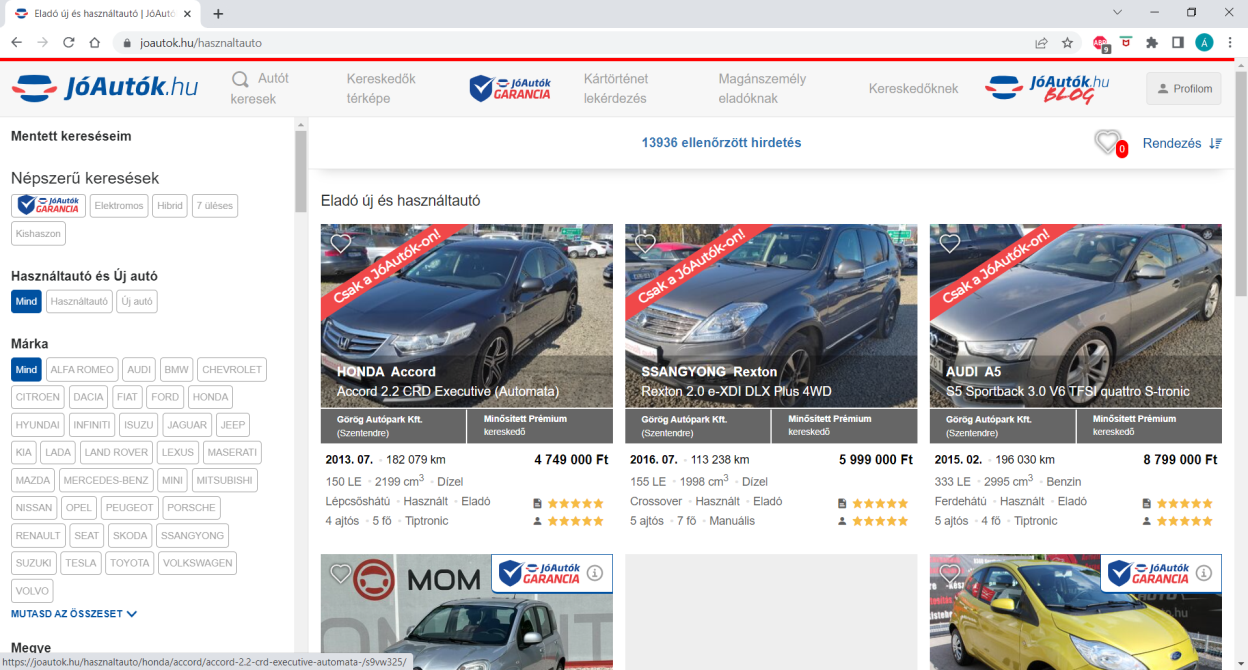
\includegraphics[scale=1]{images/joautok.png}
\caption{joautok.hu találati listája \cite{JoAuto}}
\label{fig:joautok}
\end{figure}

\subsection{Használtautó.hu}

A Használtautó.hu szerintem Magyarország legnépszerűbb használtjármű hirdető oldala, mivel itt van a legtöbb használt-autó hirdetés(2022.11.03-án Használtautó.hu-n 72 ezer hirdetés volt elérhető még a JóAutók.hu-n csak 14 ezer hirdetés állt rendelkezésre). Ezen a weboldalon személyautótól kezdve munkagépeken keresztül hajók, autóbuszok és lakókocsik vásárlására és eladására is van lehetőség, tehát egy nagyon széles körű weboldalról beszélünk amit a \ref{fig:hasznaltauto}. ábra is szemléltet.

A JóAutóktól eltérően itt először meg tudjuk adni a keresési feltételeinket, hogy milyen autók hirdetéseit szeretnénk látni.

\begin{figure}[h]
\centering
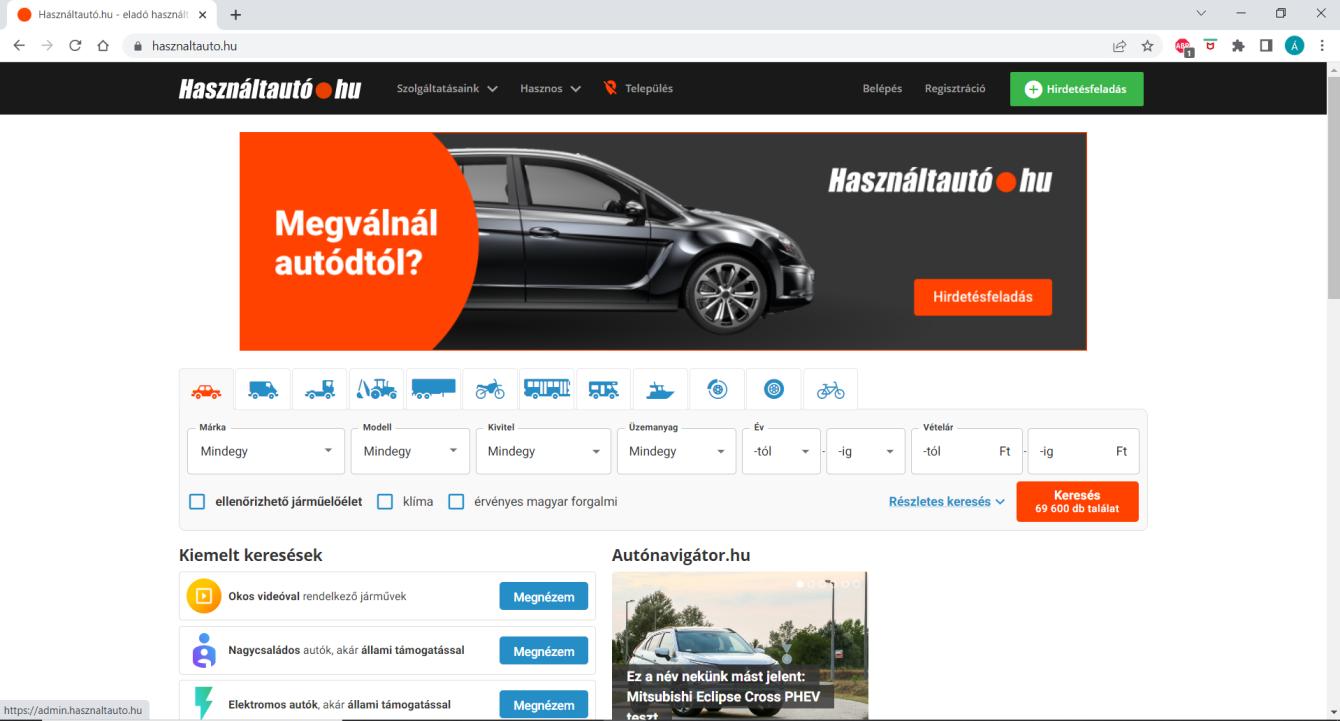
\includegraphics[scale=0.8]{images/hasznaltauto.png}
\caption{hasznaltauto.hu főoldala\cite{Hasznaltauto}}
\label{fig:hasznaltauto}
\end{figure}
\newpage

Használtautó.hu-nak van egy olyan funkciója, amit úgy hívnak, hogy „Okos videó”, ami azt jelenti, hogy egy rövid kis videóban végig mutatja az autóról feltöltött képeket, közben megjelennek az autó paraméterei is, hogy mennyi kilométer van benne, milyen évjáratú, milyen üzemanyagot fogyaszt. 

\Section{Aggregáló oldal}

Az aggregáló oldalaknak az a lényege, hogy több oldalról gyűjtik össze az információkat egy témáról, árukról, egy adott termékről az összes elérhető boltot, ahol árulják őket, és a vásárlónak lehetősége van összehasonlítani az árakat, és kitudja választani a számára legmegfelelőbb boltot.

\subsection{Árukereső}

Az Árukereső pont egy olyan weboldal, ahol a látogató, össze tudja hasonlítani az árakat és a termékeket, hogy kiválassza az adott ár-kategóriában a legjobbat.

Rengetek kategória érhető el az oldalon, tehát szinte bármi megtalálható rajta, amit csak szeretne venni egy fogyasztó, mint például:

\begin{itemize}
\item ajándékok,
\item hobbi felszerelések,
\item játékok,
\item műszaki cikkek.
\end{itemize}

Ezt a \ref{fig:arukereso}. ábra is szemlélteti.

\begin{figure}[h]
\centering
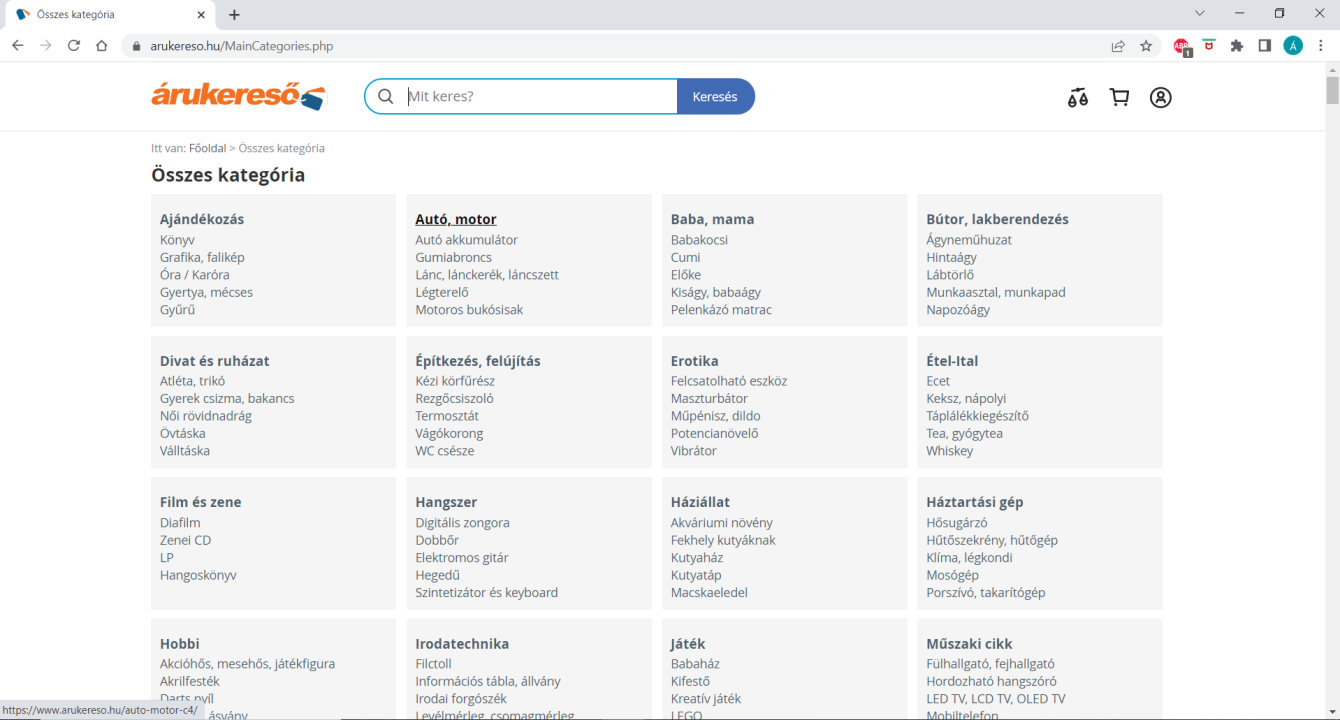
\includegraphics[scale=0.8]{images/arukereso.png}
\caption{Az árukereső kategória választója \cite{Arukereso}}.
\label{fig:arukereso}
\end{figure}
\newpage